%%%%%%%%%%%%%%%%%%%%%%%%%%%%%%%%%%%%%%%%%%%%%%%%%%%%%%%
%                File: OpEx_temp.tex                  %
%                  Date: Sept. 2, 2009                %
%                                                     %
%           LaTeX template file for use with          %
%           OSA's journal Optics Express              %
%                                                     %
%  send comments to Jennifer Mayfield, jmayfi@osa.org %
%                                                     %
% This file requires style file, opex3.sty, under     %
%              the LaTeX article class                %
%                                                     %
%   \documentclass[10pt,letterpaper]{article}         %
%   \usepackage{opex3}                                %
%                                                     %
% Note that our online submission system does not     %
% currently process PDFLaTeX; if PDFLaTeX must be     %
% used, pls. contact OpEx staff, and we will process  %
% manually                                            %
%                                                     %
%                                                     %
%       (c) 2009 Optical Society of America           %
%%%%%%%%%%%%%%%%%%%%%%%%%%%%%%%%%%%%%%%%%%%%%%%%%%%%%%%

%%%%%%%%%%%%%%%%%%%%%%% preamble %%%%%%%%%%%%%%%%%%%%%%%%%%%
\documentclass[10pt,letterpaper]{article}
\usepackage{{../lib/opex3}}
%\usepackage{{../lib/penarandaY}}
\graphicspath{{../Pictures/}}
\usepackage{caption}
\usepackage{subcaption}
\usepackage{amsmath} % Required for equation and aligned environments
\usepackage{hyperref}
\RequirePackage{numprint}

%\usepackage{ae} %%for Computer Modern fonts

%%%%%%%%%%%%%%%%%%%%%%% begin %%%%%%%%%%%%%%%%%%%%%%%%%%%%%%
\begin{document}

%%%%%%%%%%%%%%%%%% title page information %%%%%%%%%%%%%%%%%%
\title{Chromatic Objective Design for Extended Depth of Focus \textit{(EDOF)}}

\author{M. Yohan Penaranda, M. Gostiaux Gabriel}

\address{M. Gabriel Gostiaux, Master of Science student, Institute of Optics, \\ Palaiseau, 91 120, France}

\email{gabriel.gostiaux@institutoptique.fr} %% email address is required

%\homepage{https://github.com/GabrielGst?tab=repositories} %% author's URL, if desired

%%%%%%%%%%%%%%%%%%% abstract and OCIS codes %%%%%%%%%%%%%%%%
%% [use \begin{abstract*}...\end{abstract*} if exempt from copyright]

\begin{abstract*}
This study introduces basic concepts of co-design to implement and optimize a chromatic imaging system dedicated to EDOF, in the pursuit of post-tratment using high-frequency transfer algorithm to enhance RGB image resolution.
%\linebreak
\hfill \break

\textbf{Keywords:} EDOF, high frequency transfer, chromatic imaging system.
%\linebreak

\end{abstract*}

\ocis{(000.0000) General.} % REPLACE WITH CORRECT OCIS CODES FOR YOUR ARTICLE

%%%%%%%%%%%%%%%%%%%%%%% References %%%%%%%%%%%%%%%%%%%%%%%%%
\begin{thebibliography}{99}

%\bibitem{labwork} F. Goudail, D. Bloch, O. Leveque, ``FED labworks and projects,'' IOGS {\bf lab 3-4-5,} (2024)
\bibitem{trouve} P. TROUVE, ``Co-conception pourr la mesure 3D,'' IOGS, 11--25 (2024).
\bibitem{TNT+08} C.L. Tisse, H.P. Nguyen, R. Tessières, M. Pyanet, and F. Guichard. ``Extended
depth-of-field (EDoF) using sharpness transport across colour channels,'' In
Society of Photo-Optical Instrumentation Engineers (SPIE) Conference Series, {\bf volume 7061, page 4} (2008).

\end{thebibliography}

%%%%%%%%%%%%%%%%%%%%%%%%%%  body  %%%%%%%%%%%%%%%%%%%%%%%%%%
\section{Introduction}
One of the many objectives of co-design is to simulate optical designs in order to optimize costs through reducing the number of elements of the optical chain of a system. It is also possible to replace costly elements with hybrid ones, integrating signal and image processing in the system.

Here, we will focus on two methods for extended depth of focus. The first section deals with the design of a EDOF algorithm which uses high frequency transfer, applied to real images acquired with a chromatic imaging system. The second section will dive into the modelling of such a chromatic system. We will see how optimizing the curvature radius and the focus, can be monitored by the criteria of maximizing the \textbf{object-camera} range within which at least one of the channels is resolved. This is actually equivalent to maximizing the union of the depths of focus of the three RGB channels of a chromatic camera within a range of interest.

\begin{equation}\label{eqn:gdof}
    G D O F=L \cap\left(\cup_{i \in R, V, B} D o F_i\right)
\end{equation}


\section{High Frequency Transfer}
To design the right chromatic imaging system, we should first focus on the post-treatment process. Here, the method presented in \cite{TNT+08}consist in adding to each color channel the high frequencies of all the other channels, \textbf{weighted by the resolution level of each channel}. This can be expressed as :

\begin{equation}\label{eqn:HFT}
    y_{c}^{EDOF} = y_{c}^{init} + \alpha . HF_R + \beta . HF_G + \gamma . HF_B
\end{equation}


\begin{figure}[h]
	\centering
	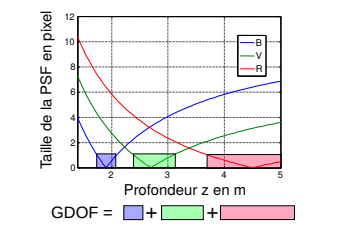
\includegraphics[scale=0.7]{HFRs.png}
	\caption{illustration of the Generalized Depth of Focus concept}
	\label{fig:gdof}
\end{figure}


We will see how the resolution can be improved regarding the depth of focus, even after the acquisition of the image. One can see the original picture on fig. \ref{sub@fig:origin} and the enhanced picture on fig. \ref{sub@fig:edof} .

\begin{figure}[h]
    \centering
    \subfloat[Original picture]{
        \centering
        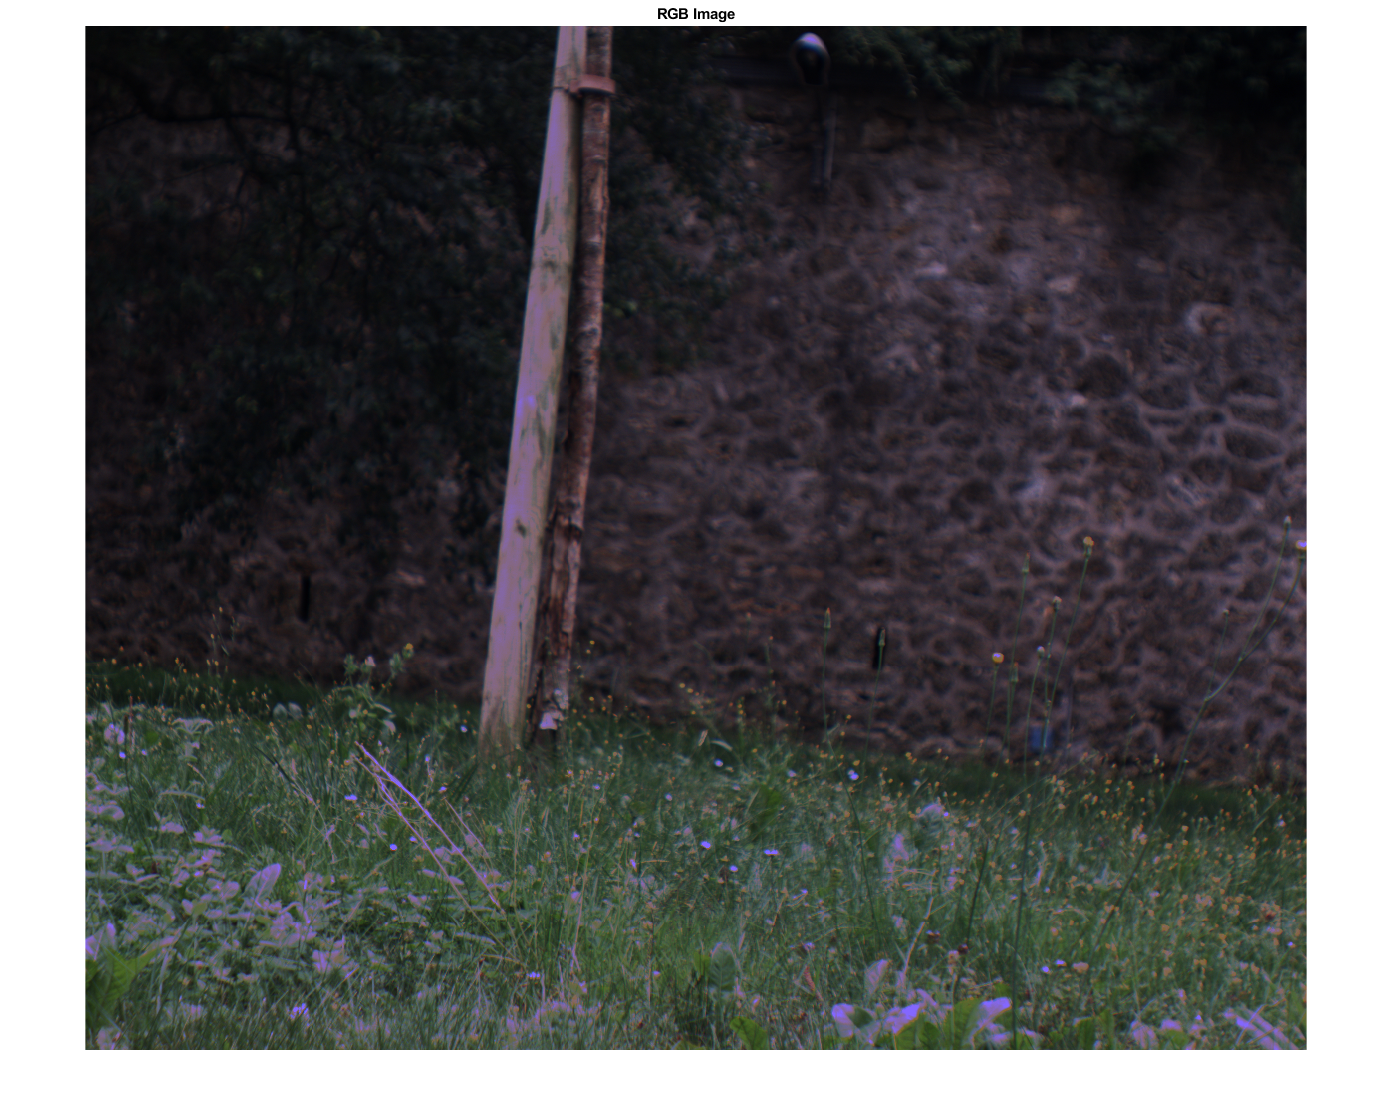
\includegraphics[width=0.3\textwidth]{Original picture.png}
        \label{fig:origin}
    }
	\subfloat[Optimized picture]{
		\centering
        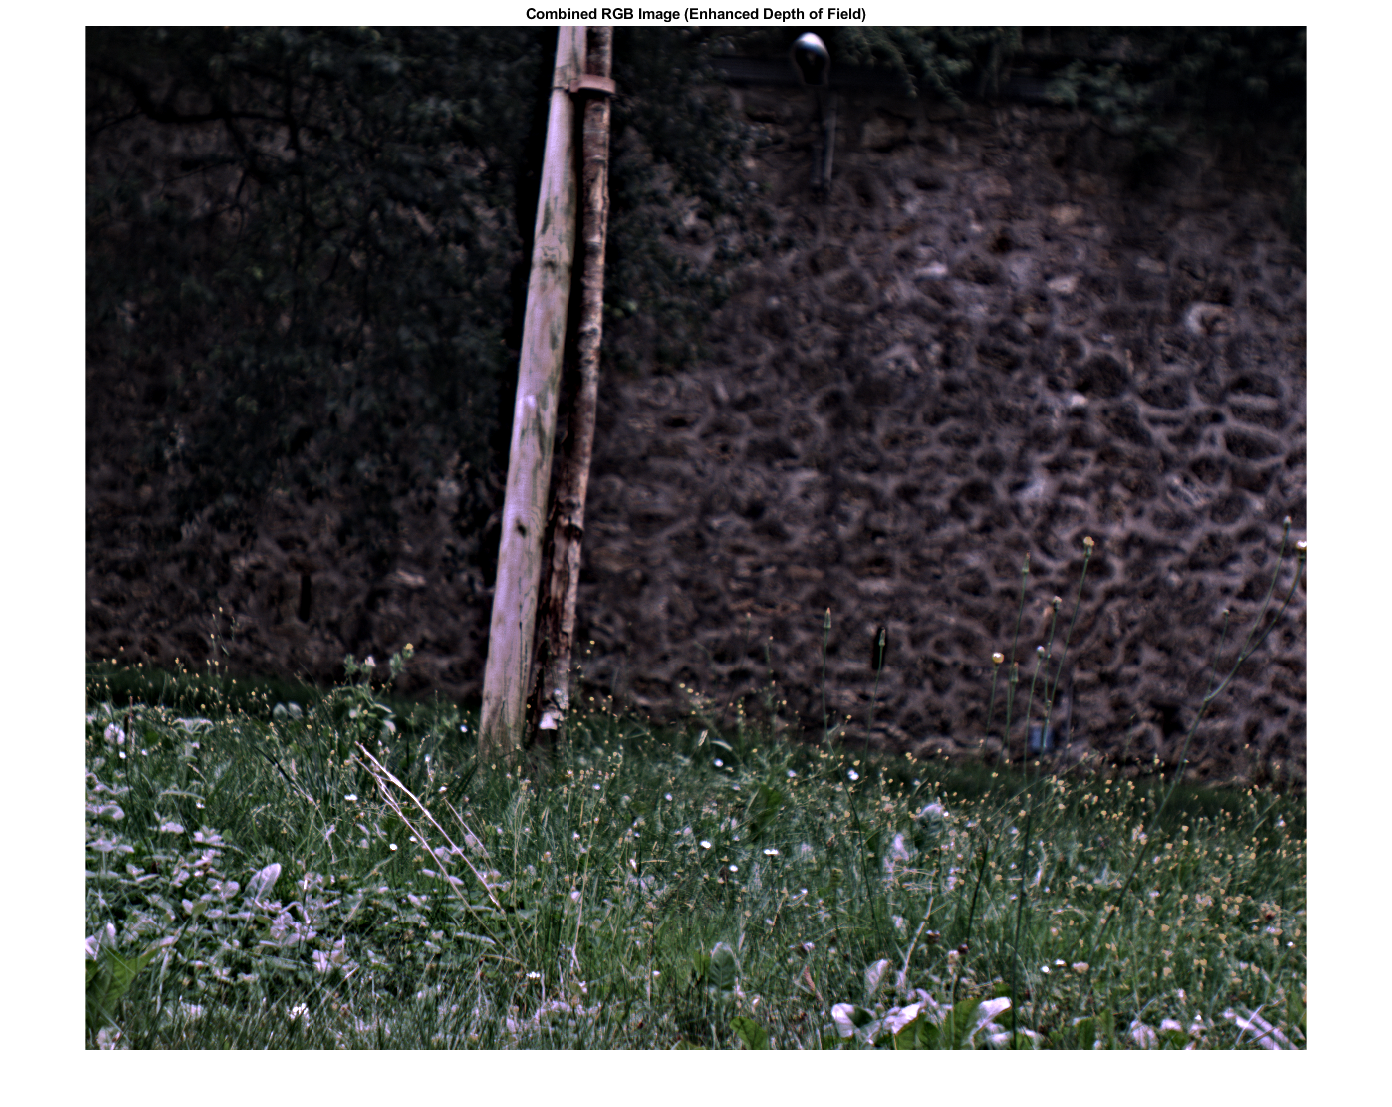
\includegraphics[width=0.3\textwidth]{Final EDOF.png}
        \label{fig:edof}
    }
	\caption{High Frequency Transfer}
\end{figure}

We will talk about the multiple improvements in resolution at the end of the section, and first focus on presenting the method that led to the EDOF picture, presenting the computation of the weight factors $\alpha, \beta, \gamma$.

\subsection*{Coefficient computation}
We start by separating the three R, G, B channels that constitute the image, and we look at them separately : one can figure that the best resolution is obtained for the red channel, and the worst for the blue channel. This is caused by chromatic dispersion induced by the glass used in the lenses of the imaging system.

\begin{figure}[h]
	\centering
	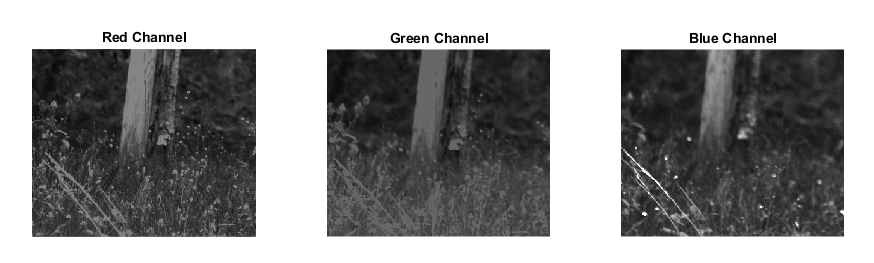
\includegraphics[scale=0.45]{Channels Original and Blured DOF.png}
	\caption{Blured blue and green channels}
	\label{fig:blured-channels}
\end{figure}

Let us now compute the coefficients $\alpha,\beta,\gamma$ thanks to the expression of the gradients computed on the different channels. We use to the formula:

$$
\begin{aligned}
\alpha & =\frac{\left\|\Delta_{y_R}\right\|^2}{\left\|\Delta_{y_R}\right\|^2+\left\|\Delta_{y_V}\right\|^2+\left\|\Delta_{y_B}\right\|^2} \\ 
\beta & =\frac{\left\|\Delta_{y_V}\right\|^2}{\left\|\Delta_{y_R}\right\|^2+\left\|\Delta_{y_V}\right\|^2+\left\|\Delta_{y_B}\right\|^2} \\ 
\gamma & =\frac{\left\|\Delta_{y_B}\right\|^2}{\left\|\Delta_{y_R}\right\|^2+\left\|\Delta_{y_V}\right\|^2+\left\|\Delta_{y_B}\right\|^2}\end{aligned}
$$

We apply a mean filter in order to smooth those gradients and work with the surroundings of the details contained in the image. The result of the mean filter can be seen on the right side of Fig. \ref{fig:gradients} : the image presents the surroundings of the high variating contrast zones that can be seen on the left side of Fig. \ref{fig:gradients}.

\begin{figure}[h]
    \centering
    \subfloat[Gradients of each channels]{
        \centering
        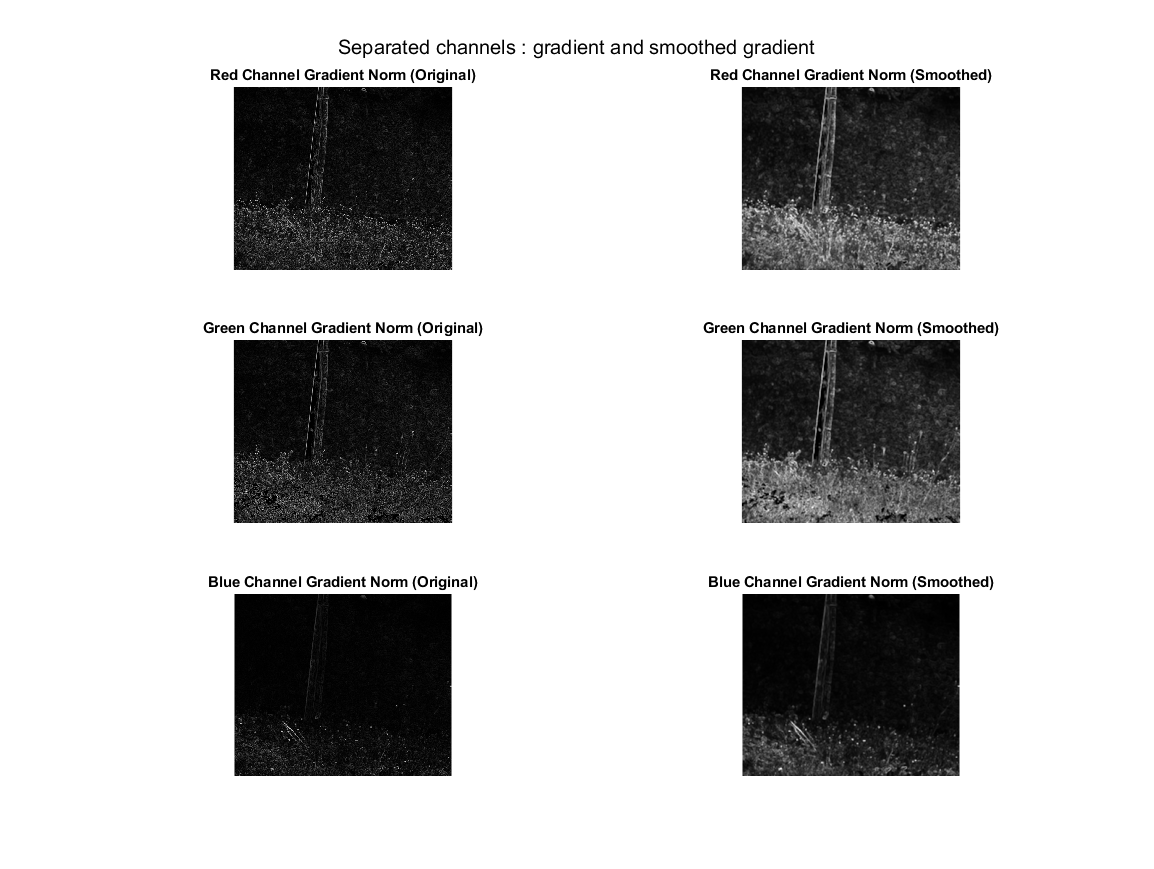
\includegraphics[width=0.38\textwidth]{Channels Gradient Norms (orig vs smothed).png}
        \label{fig:gradients}
    }
	\subfloat[High frequency channels]{
		\centering
        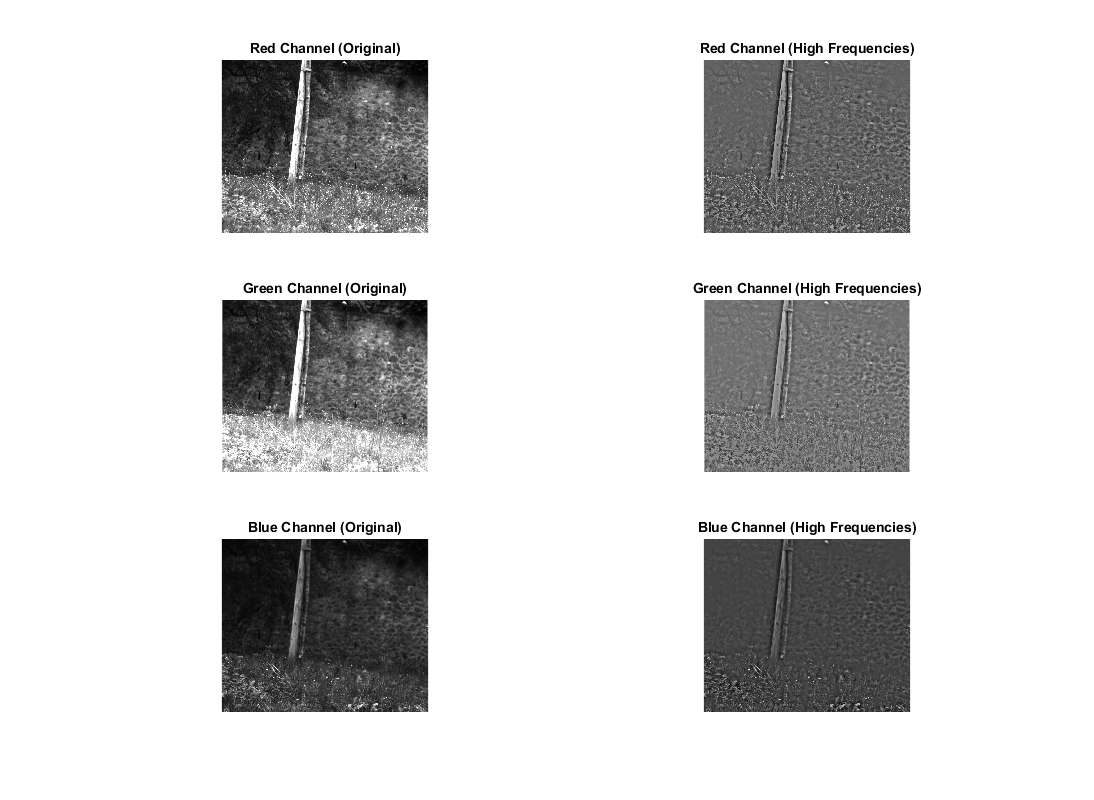
\includegraphics[width=0.38\textwidth]{Channels High Freq.png}
        \label{fig:hfc}
    }
	\caption{High Frequency Transfer}
\end{figure}

Let us then extract the high frequency components of each channels, in order to apply the equation \ref{eqn:HFT} and compute the resolved channels. In this purpose, we compute the convolution of the channels with a large PSF ( size $s = \numprint[pix]{50}$) to obtain the low frequencies.  We then substract them from the initial channel to obtain the remaining high frequencies, as can be seen on fig. \ref{fig:hfc}.

We thus obtain three corrected channels, as can be seein on fig. \ref{fig:edof-channels} .

\begin{figure}[h]
    \centering
    \subfloat[EDOF channels]{
        \centering
        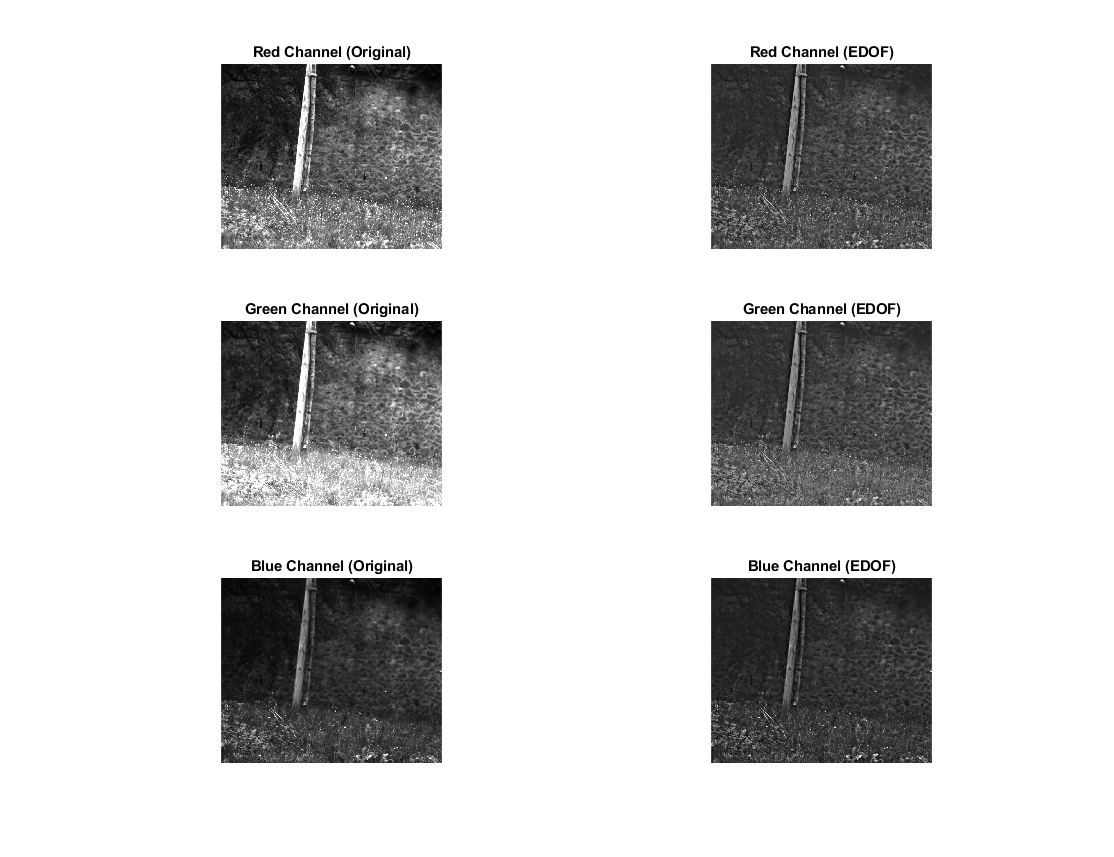
\includegraphics[width=0.37\textwidth]{EDOF channels.png}
        \label{fig:edof-channels}
    }
	\subfloat[EDOF channels (zoomed)]{
		\centering
        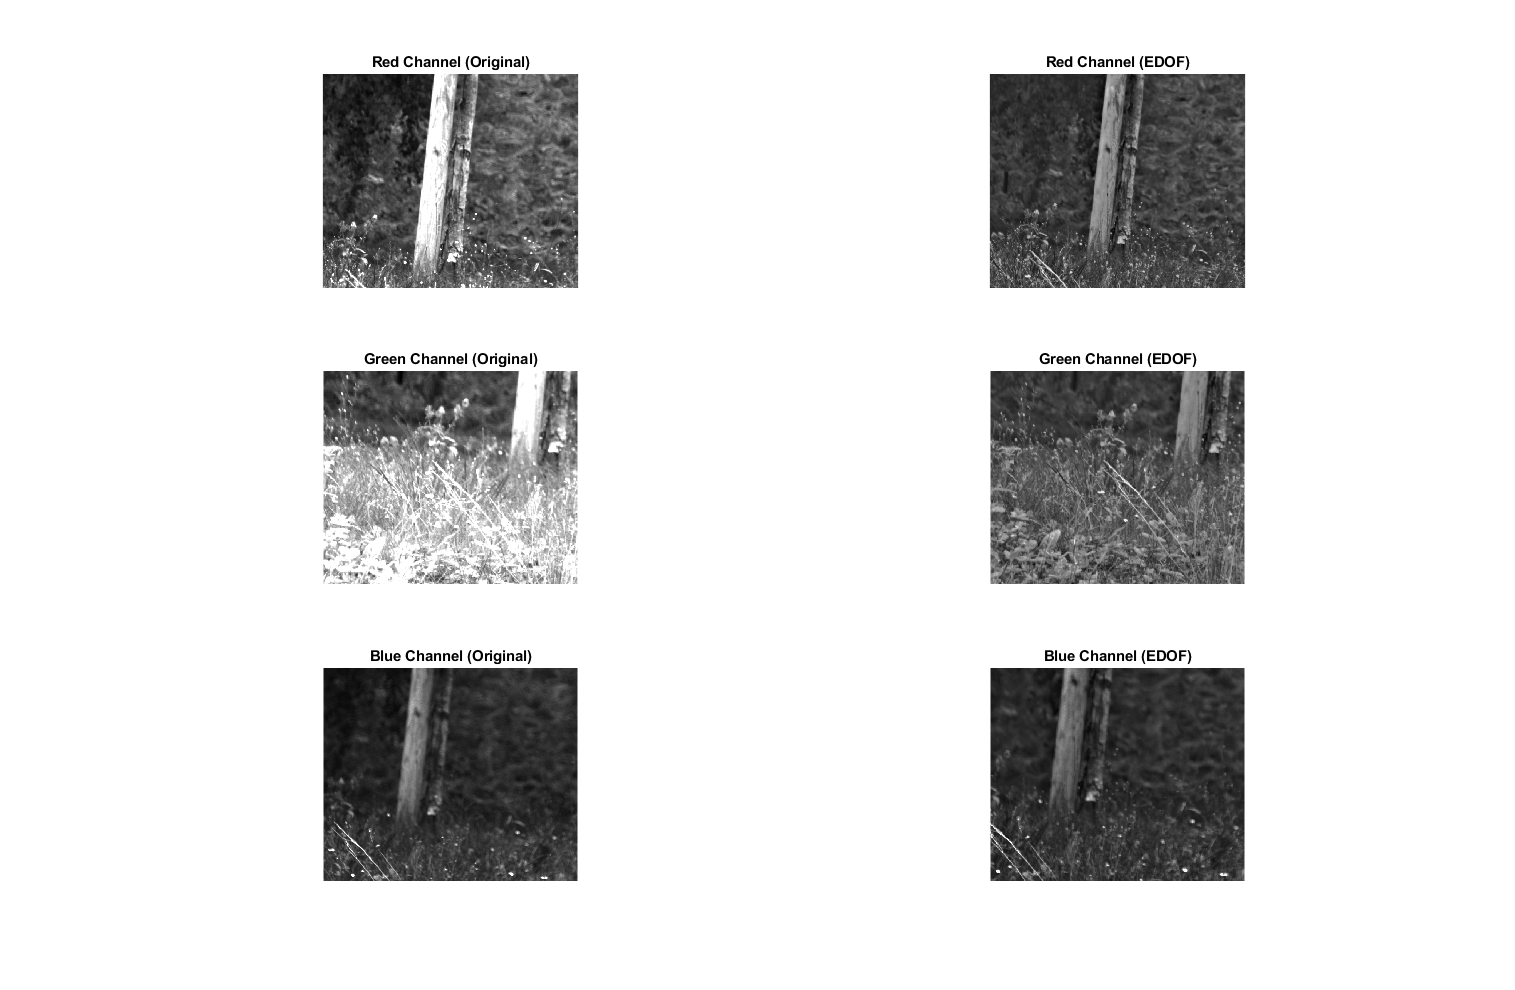
\includegraphics[width=0.44\textwidth]{EDOF channels zoomed.png}
        \label{fig:edof-channels-zoomed}
    }
	\caption{High Frequency Transfer}
\end{figure}
\pagebreak

\subsection*{Results and discussion}
Applying the high frequency transfer algorithm to an image helps improving chromatic defocus, but it also seems to flatten the image by reducing saturation (mostly on the green channel).

In regard of fig. \ref{fig:cutoff} on which are presented the EDOF pictures according to the cutoff frequency of the lowpass filter (which parameter is the size of the PSF), one can see that the effect of the HF transfer is to emphasize the details of the high frequencies which have not been filtered, thus degrading contrast of highly detailed zones over the image (such as the bark of the tree). Thus, one could define a mid-range threshold that would lead to a resolution trade-off between highly-detailed and poorly-detailed zones. One could also apply a different threshold according to a spatial parameter representing the level of detail of one zone in the image.

\begin{figure}[h]
	\centering
	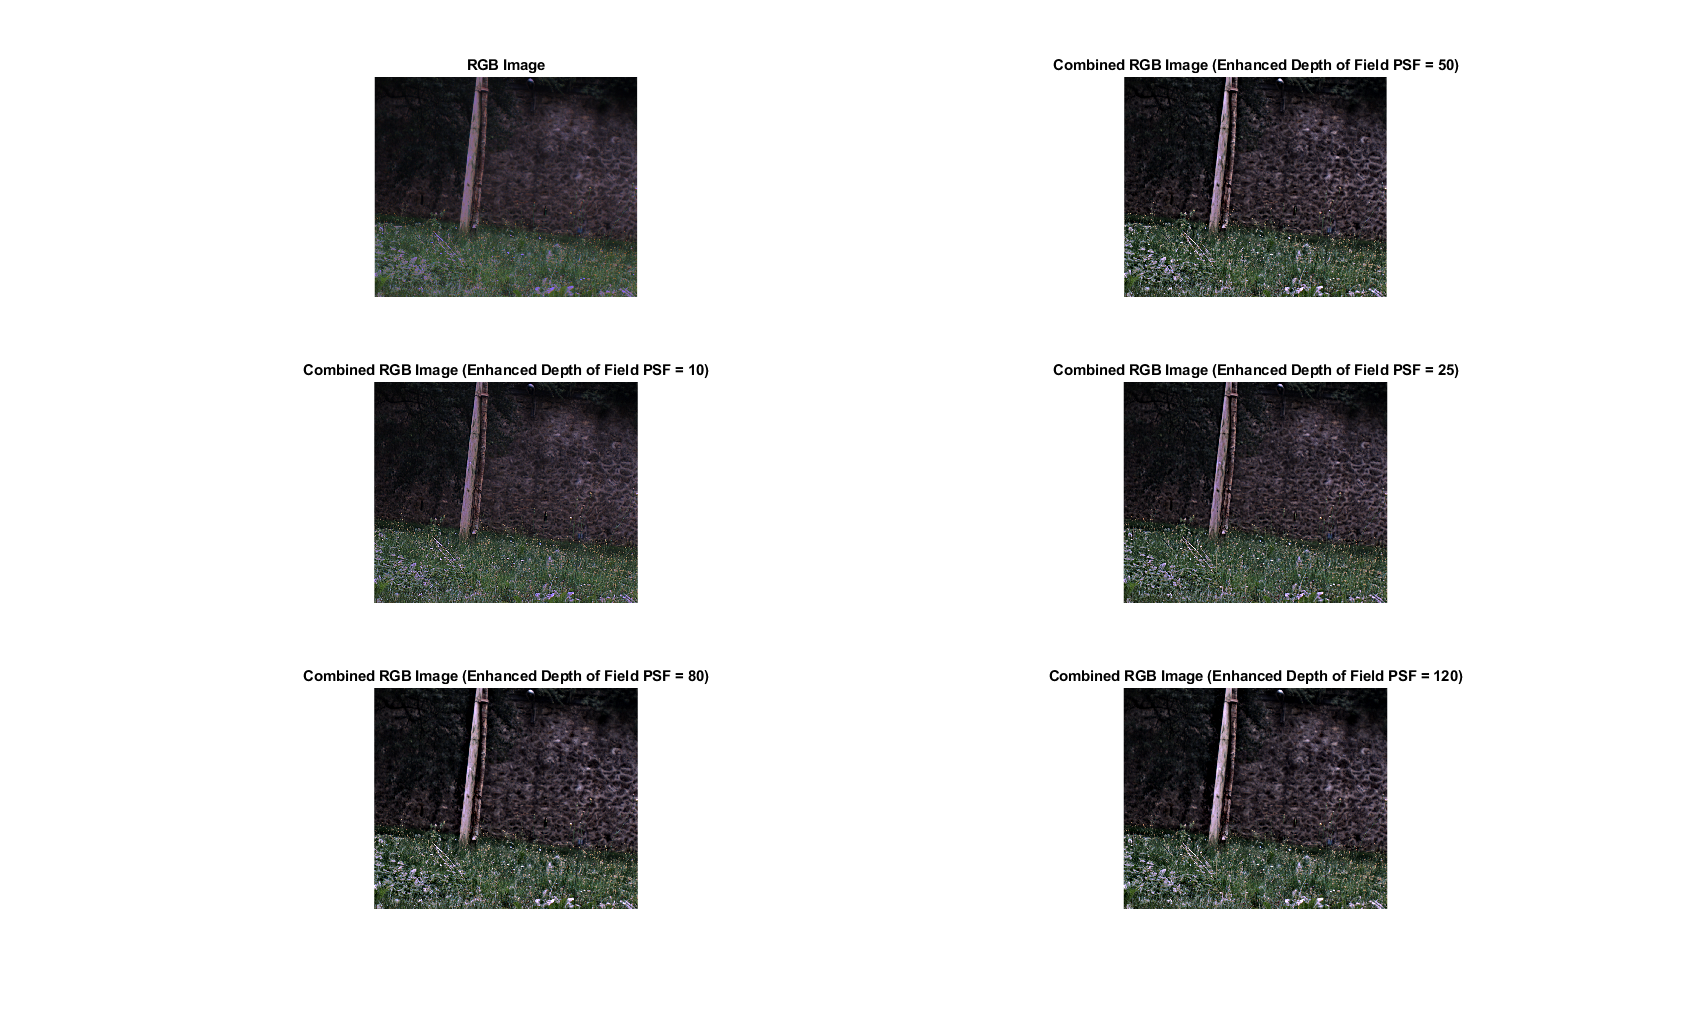
\includegraphics[scale=0.25]{PSF variating EDOF RGB.png}
	\caption{EDOF, variating frequency cutoff}
	\label{fig:cutoff}
\end{figure}


\section{Chromatic Imaging Design}
The first step in the co-design process involves modeling the imaging system to estimate the performance criterion based on the parameters to be optimized.

To achieve this, it is necessary to develop functions that simulate variations in defocus blur for both a conventional optical system and a chromatic optical system. Next, the goal is to compute the performance criterion - specifically, the generalized depth of field - as a function of the imaging system parameters.

Finally, these functions will be used to optimize first the radius of curvature of the chromatic doublet, and then both the radius of curvature and the focusing mechanism of the imaging system.

\subsection*{Ideal lens}
We first consider a conventional camera with the following generic parameters: focal length $f' = 25 \, \text{mm}$, aperture number $N = 2.8$, and pixel size $t_{\text{pix}} = 5 \, \mu\text{m}$. The object is located between 1 and 5 meters from the camera. Fig. \ref{fig:ideal-lens} illustrates the parameters of this model.

\begin{figure}[h]
	\centering
	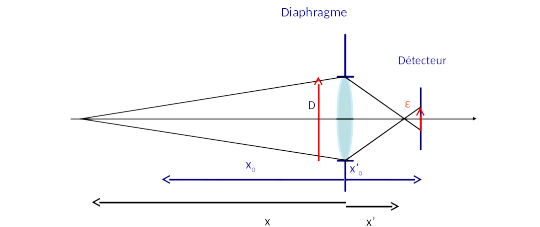
\includegraphics[scale=0.75]{Ideal_lens.png}
	\caption{Depth of focus for an ideal lens}
	\label{fig:ideal-lens}
\end{figure}
\pagebreak

We recall the formula that characterizes the size of the defocus blur as a function of the optical parameters ($f'$: focal length, $D$: lens diameter) and the depth $x$:

\begin{equation}\label{eqn:dof}
    \epsilon = D x'_0 \left( \frac{1}{f'} + \frac{1}{x} - \frac{1}{x'_0} \right)
\end{equation}
    

In the context of an object located at $x=\numprint[m]{-2}$, we can compute the location of the detector for paraxial rays :

\begin{align}
    \frac{1}{x'_0} - \frac{1}{x_0} &= \frac{1}{f'}\\
    x'_0=\frac{1}{\frac{1}{f'} + \frac{1}{x_0}} &= \numprint[mm]{25.3}
\end{align}

We can then compute the depth of focus for this configuration :

\begin{align}
    x_{min} &= \frac{x'0}{1-\frac{x'0}{f'} + \frac{t_{px}}{D}} = \numprint[m]{-2.0925}\\
    x_{max} &= \frac{x'0}{1-\frac{x'0}{f'} - \frac{t_{px}}{D}} = \numprint[m]{-1.9152}
\end{align}

Thus the depth of focus is equal to $\numprint[m]{0.1773}$. By zooming on Fig. \ref{fig:ideal-def}, we can find a similar result when looking on x-axis minimum and maximum values corresponding to y-values inferior to 1 pixel. this result correspond to the output of the $\operatorname{IsInDoF}$ function computing the depth of focus as the total length of the union of the depth of focus of the three channels.


\subsection*{Chromatic lens}
We now introduce chromatic dispersion and consider a chromatic optical system such that: $f_R = 25.1 \, \text{mm}$, $f_V = 25 \, \text{mm}$, and $f_B = 24.8 \, \text{mm}$. The aperture number is still $N = 2.8$, and the pixel size is $t_{\text{pix}} = 5 \, \mu\text{m}$. The object is still located between 1 and 5 meters.

A function was developed to calculate the size of the defocus blur for the three color channels (R, G, B) as a function of depth and the parameters $f_R, f_V, f_B, N, t_{\text{pix}},$ and $x_0'$. The sensor was positioned such that the focal plane $x_0$ aligns with the focus of the green channel (denoted as $x_0^V$).

The defocus blur variations for the RGB channels of the camera were then plotted on the same graph, showing how the blur size changes with depth (see Fig. \ref{fig:def-blur}).

\begin{figure}[h]
    \centering
    \subfloat[Ideal lens]{
        \centering
        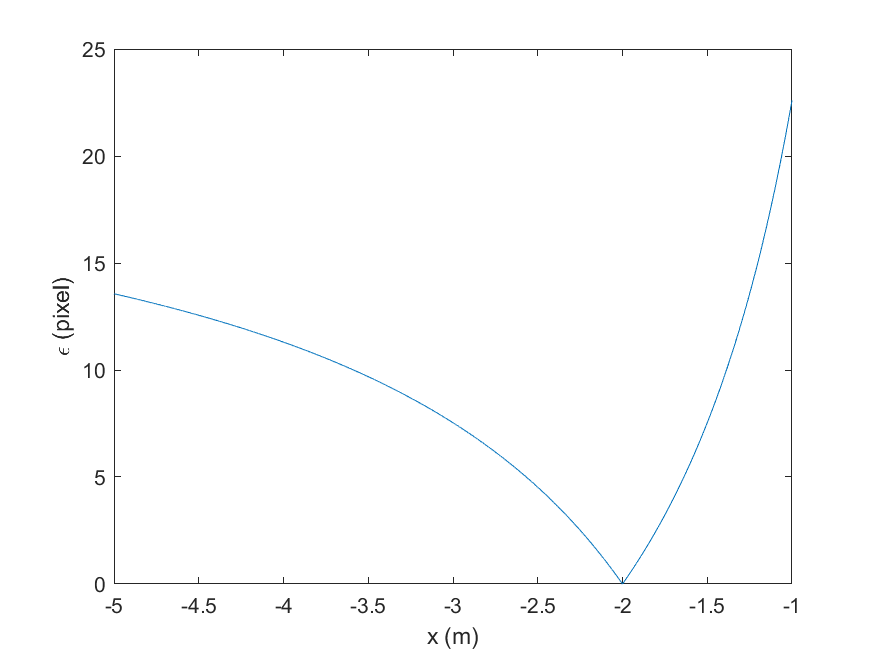
\includegraphics[width=0.45\textwidth]{flou_defocalisation_conventionnelle.png}
        \label{fig:ideal-def}
    }
	\subfloat[Chromatic lens]{
		\centering
        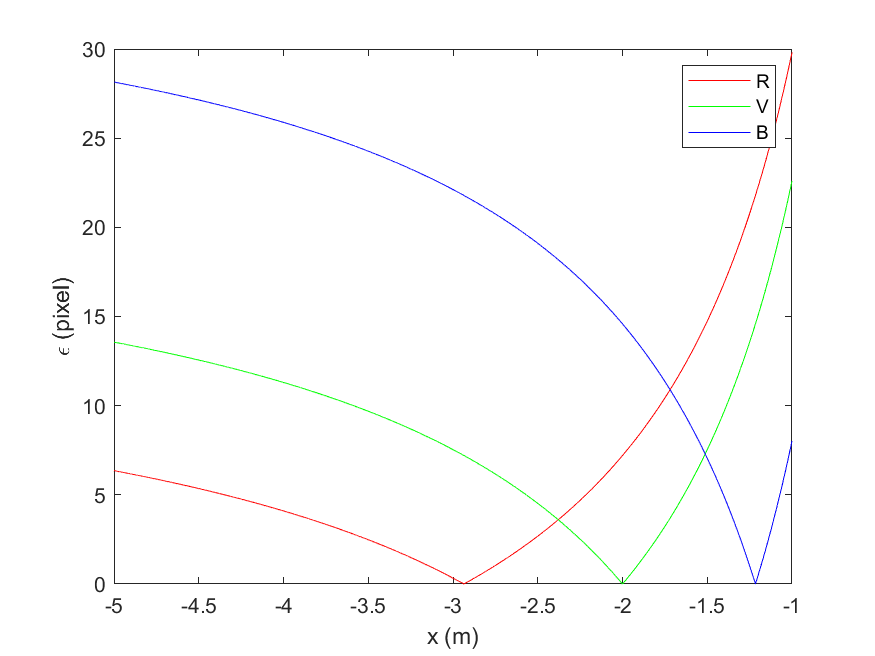
\includegraphics[width=0.45\textwidth]{flou_defocalisation_RVB.png}
        \label{fig:def-blur}
    }
	\caption{Depth of focus according to the distance of an object}
\end{figure}

\subsection*{Performance}
The function $\operatorname{IsInDoF}$ created before was used to construct a new function that, given a depth vector, calculates the generalized depth of field of a chromatic camera characterized by $f_R, f_V, f_B, N, t_{\text{pix}},$ and $x_0'$. 

To achieve this, the union function, which computes the union of two vectors without repetition, was utilized. Finally, the generalized depth of field for this system was calculated.

The function gives the value of the generalized depth of field for this system, which is $\numprint[m]{0.625}$ and is consistent with the graphic plotted on Fig. \ref{fig:def-blur}.
Table \ref{tab:prof_champ_RVB} details the calculation of depth of field for the three channels.
\begin{table}[h] 
    \centering
    \begin{tabular}{|l|c|c|c|} \cline{2-4}
   \multicolumn{1}{c|}{}  &  \multicolumn{3}{c|}{Bornes (m)} \\ \cline{2-4}
   \multicolumn{1}{c|}{}  &  Rouge  &  Vert & Bleu \\ \hline
   Minimum & $\numprint{-3.139}$ & $\numprint{-2.093}$ & $\numprint{-1.250}$  \\ \hline
   Maximum & $\numprint{-2.757}$ & $\numprint{-1.915}$ & $\numprint{-1.184}$ \\ \hline
   $\Delta x$ & $\numprint{0.381}$ & $\numprint{0.177}$ & $\numprint{0.066}$ \\ \hline
   Total &  \multicolumn{3}{c|}{$\numprint{0.625}$} \\ \hline
\end{tabular}
    \caption{Generalized depth of field detail for three channels. Values are rounded to millimeters.}
    \label{tab:prof_champ_RVB}
\end{table}

\subsection*{Chromatic imaging system simulation}
Enriched by the models previously computed for an ideal lens and a chromatic one, we now consider a chromatic imager, composed of a chromatic doublet and an ideal lens as illustrated in Fig. \ref{fig:ideal-lens}. To model the dispersion effect on thhe visible spectrum, we will be using the provided function \texttt{index\_addon.m} that calculates the refractive index of the two glasses in the doublet for a given wavelength range in µm.

\paragraph{Variation of the Refractive Index\\}
The refractive indices of the two glasses in the visible spectrum are plotted on the same graph (see Fig. \ref{fig:index}). The expected observation is that the refractive indices of the two materials vary differently across the visible spectrum. This indicates chromatic dispersion, where different wavelengths are refracted at different angles. We observe an intersection point, where both index are equal. We know that means the power of the doublet will be infinite for this specific value of both indices.

\paragraph{Variation of the Focal Length\\}
We writes a function that calculates the focal length of the doublet for a given wavelength range and a curvature radius \(R\), and used it to computes the focal length over the visible spectrum. The focal length variation should be plotted for \(R = 20 \, \text{mm}\). The plot presented on Fig. \ref{fig:focal} will highlight the sensitivity of the lens system to different wavelengths, leading to the corresponding defocus.

\begin{figure}[h]
    \centering
    \subfloat[Refractive index variation]{
        \centering
        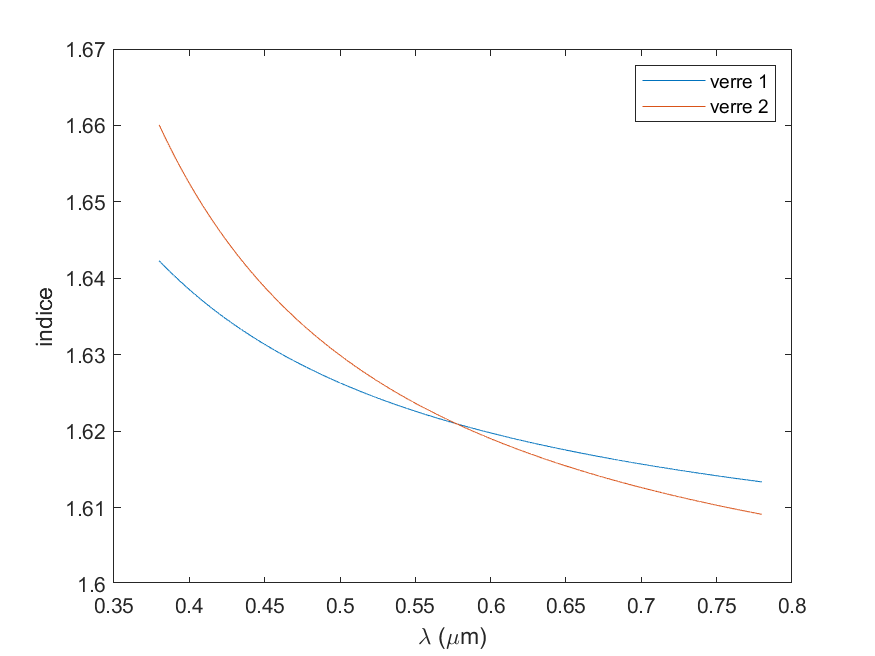
\includegraphics[width=0.4\textwidth]{indices.png}
        \label{fig:index}
    }
	\subfloat[Focal length variation]{
		\centering
        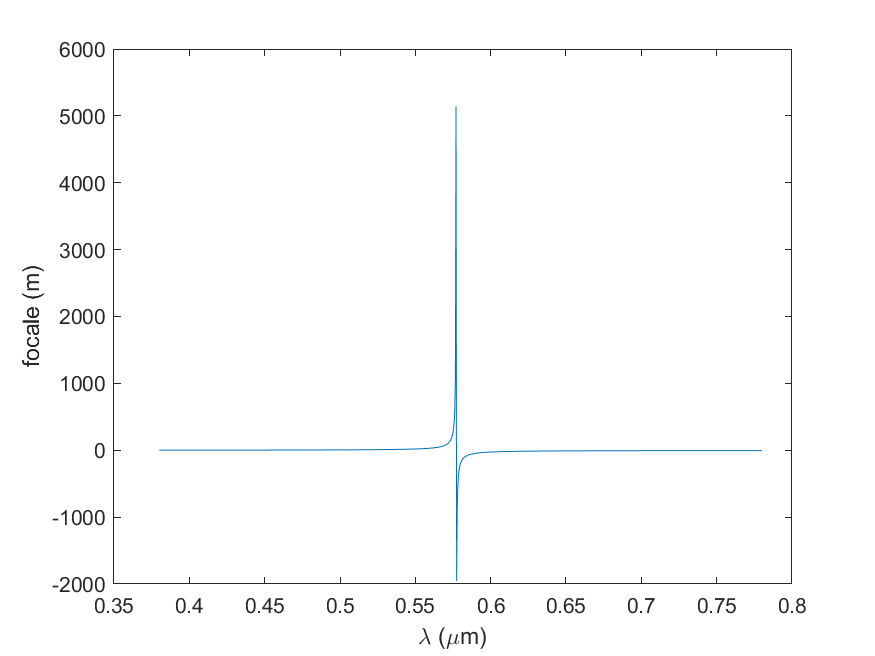
\includegraphics[width=0.4\textwidth]{focale_doublet.png}
        \label{fig:focal}
    }
	\caption{Effect of wavelength dependent refractive index association}
\end{figure}


\paragraph{Defocus Blur Calculation for the Chromatic Doublet and Ideal Lens\\}

Considering the conventional camera as a simple ideal lens (i.e. achromatic) with focal length \(f^{\prime}\), the defocus blur should be calculated for the doublet-lens system across the three channels \(R\), \(V\), and \(B\). The impact of the conventional lens will be then integrated using the .... formula.

We will still consider \(R = 20 \, \text{mm}\) and an object located within a depth range of 1 to 5 meters, in the visible spectrum. Specific wavelengths are taken as \(\lambda_R = 0.605 \, \mu \mathrm{m}\), \(\lambda_V = 0.530 \, \mu \mathrm{m}\), and \(\lambda_B = 0.465 \, \mu \mathrm{m}\). The sensor is positioned such that the green channel is in focus at \(x_0^V = -2 \, \text{m}\).

The expected result is a contraction of the doublet's chromatic dispersion through the power of the ideal lens, resulting in smaller differences between green focus and green's and red's. This analysis will reveal how defocus blur differs for different color channels underlying the impact of chromatic aberrations on image sharpness.

\begin{figure}[h]
	\centering
	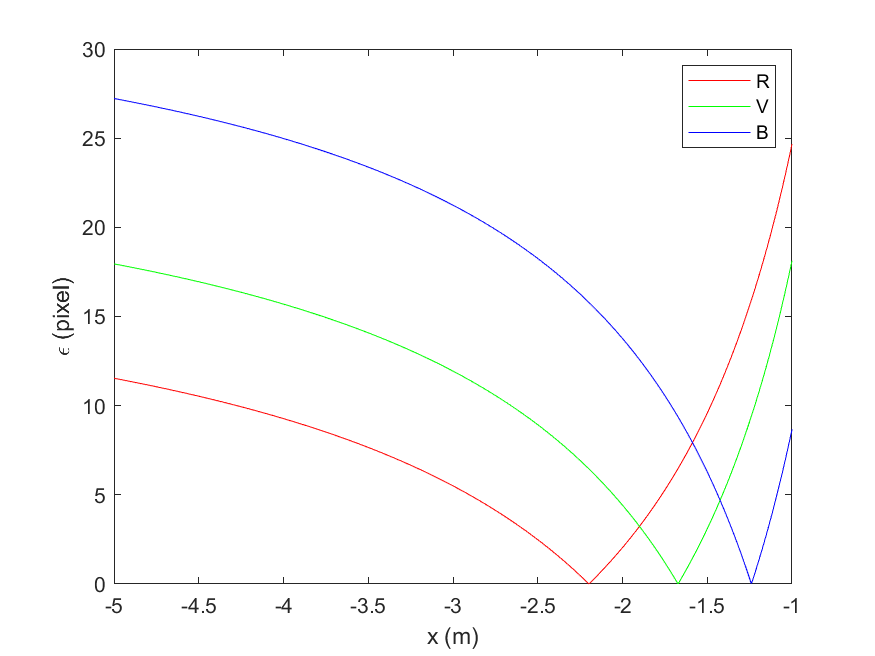
\includegraphics[scale=0.55]{flou_defocalisation_doublet_lentille_conventionnelle_RVB_optimise.png}
	\caption{Defocus blur}
	\label{fig:def-blur-2}
\end{figure}

\paragraph{Effect of Varying the Curvature Radius \(R\)\\}
The effect of varying the radius of curvature \(R\) should be explored. As \(R\) changes, it will alter the chromatic aberration and the focal length variation, which may influence the degree of defocus blur. The dependence of these parameters on \(R\) will offer insights into the optimization of lens design for minimizing chromatic effects.


\subsection*{Optimization}

\paragraph{Optimizing the Radius of Curvature of the Doublet\\}
Using the previous functions, the value of the radius of curvature of the doublet that yields the largest generalized depth of field can be determined. This optimal curvature radius corresponds to a particular chromatic aberration, characterized by the difference in focal lengths between the red and blue channels. The variations in defocus blur for the optimal setting are plotted opn Fig. \ref{fig:ratio}. Together with Fig.\ref{fig:gdof}, we can understand each zones of the charts, delimited by the violent decrease located at $R = \numprint[m]{20}$ and $R = \numprint[m]{60}$.

Those decrease occurs when the depth of focus of one color, blue or red, meets green's depth of focus, resulting in the decrease of the total depth of focus computed by the operator $\operatorname{IsInDoF}$. In the end, only the depth of focus of the green channel remain, as can be seen for $R$ values ranging above $R = \numprint[m]{60}$. In reality, each depth of focus are overlaying. Looking at Fig. \ref{fig:def-blur} and its variation with $R$, we can understand the effect of a change in the difference between the focus of the blue or red channel, and the green one, on the depth of focus of the blue or red channel. Focusing further increases the depth of focus, resulting in the increase of the GDOF, and closer reduces it. However getting closer to green's depth of focus will ultimately results in those two overlaying, resulting on the decrease of the GDOF. That's why we can observe two increases and two decreases.

Ultimately, we choose $R = \numprint[mm]{63}$ corresponding to the second maximum of the ratio function as the optimal $R$, and plot on Fig. \ref{fig:curv-opt} the resulting GDOF. We thus add $\numprint[cm]{6.01}$ to the depth of focus with this method, which represent around 7\% of the previous GDOF.

\begin{figure}[h]
    \centering
    \subfloat[Curvature radius optimization results]{
        \centering
        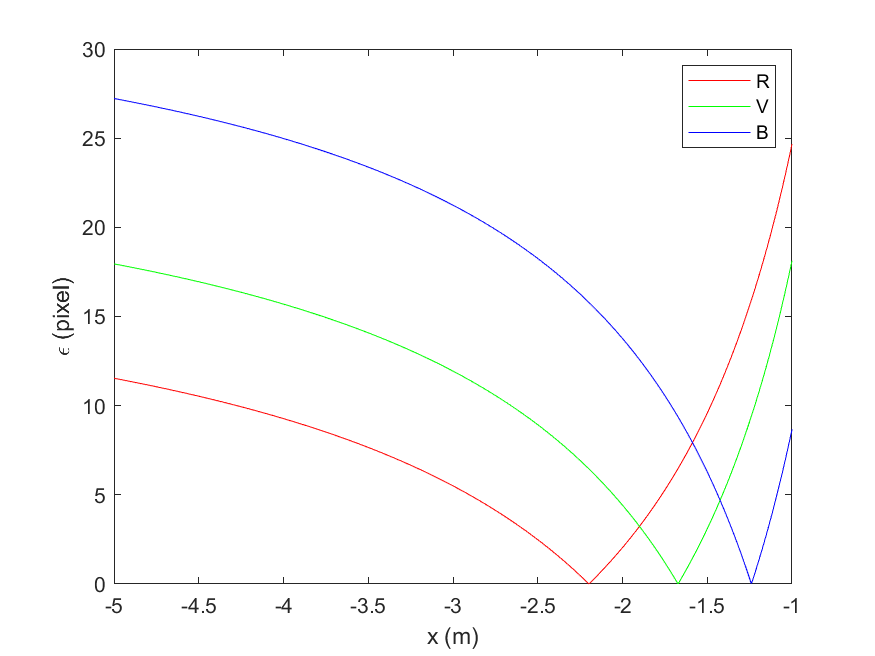
\includegraphics[width=0.4\textwidth]{flou_defocalisation_doublet_lentille_conventionnelle_RVB_optimise.png}
        \label{fig:curv-opt}
    }
	\subfloat[Ratio]{
		\centering
        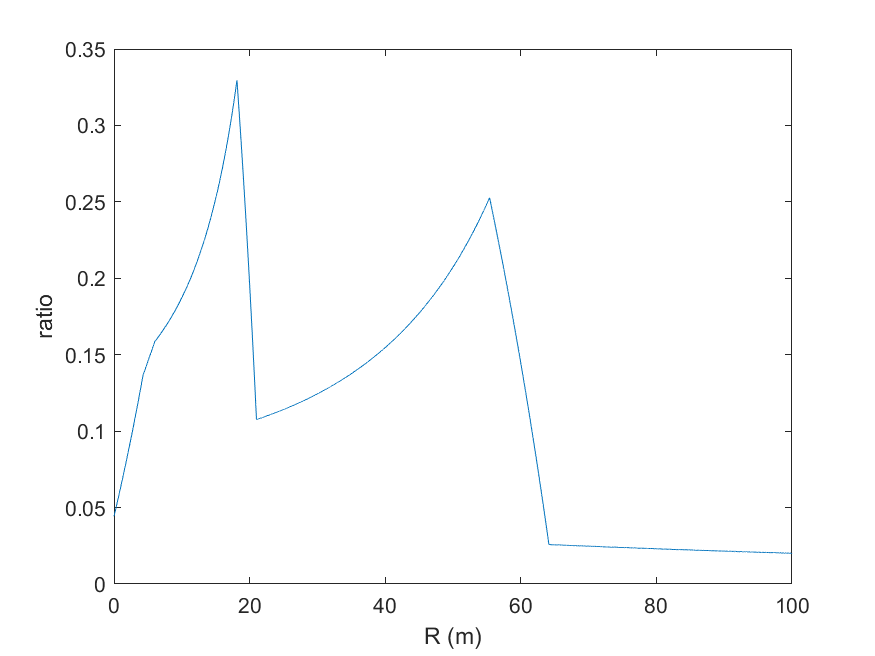
\includegraphics[width=0.4\textwidth]{Ratio_systeme.png}
        \label{fig:ratio}
    }
	\caption{Curvature radius optimization}
\end{figure}

\paragraph{Optimizing the Position of the Sensor}
Locking the curvature radius at its optimised position allows the scan of the position of the detector to maximise the ratio function. This scan is plot Fig. \ref{fig:optimisation_capteur} and shows a maximum for $\numprint[mm]{25.1}$. For this value, the GDOF changes from $\numprint[cm]{46}$ to $\numprint[m]{1.92}$ which is 400\% more than the radius-optimized setup However this is the potential depth of focus after post-processing with HFR algorithm.


\begin{figure}[h]
    \centering
    \subfloat[GDOF ratio, function of detector position]{
        \centering
        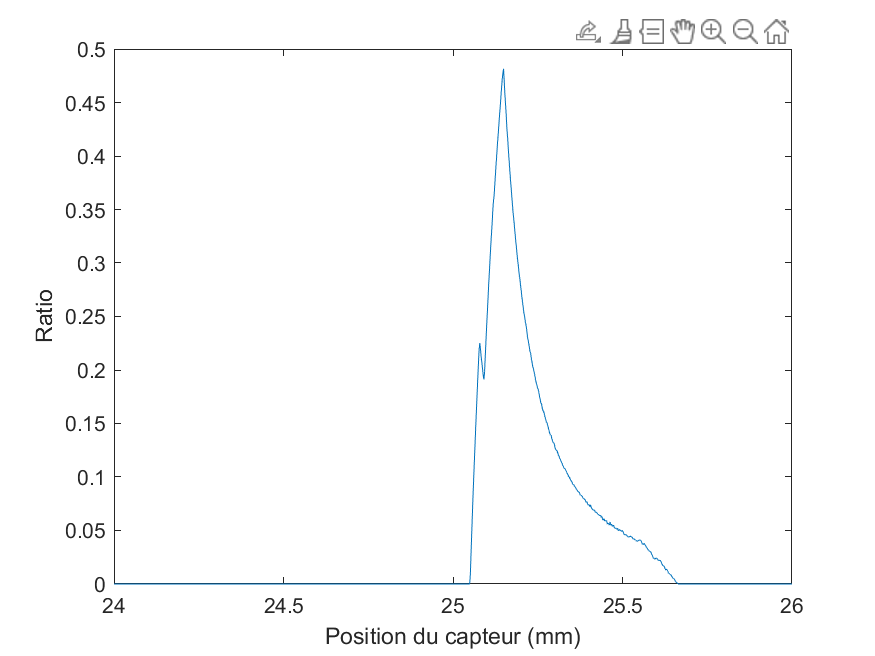
\includegraphics[width=0.4\textwidth]{optimisation_capteur.png}
        \label{fig:optimisation_capteur}
    }
	\subfloat[Final EDOF GDOF]{
		\centering
        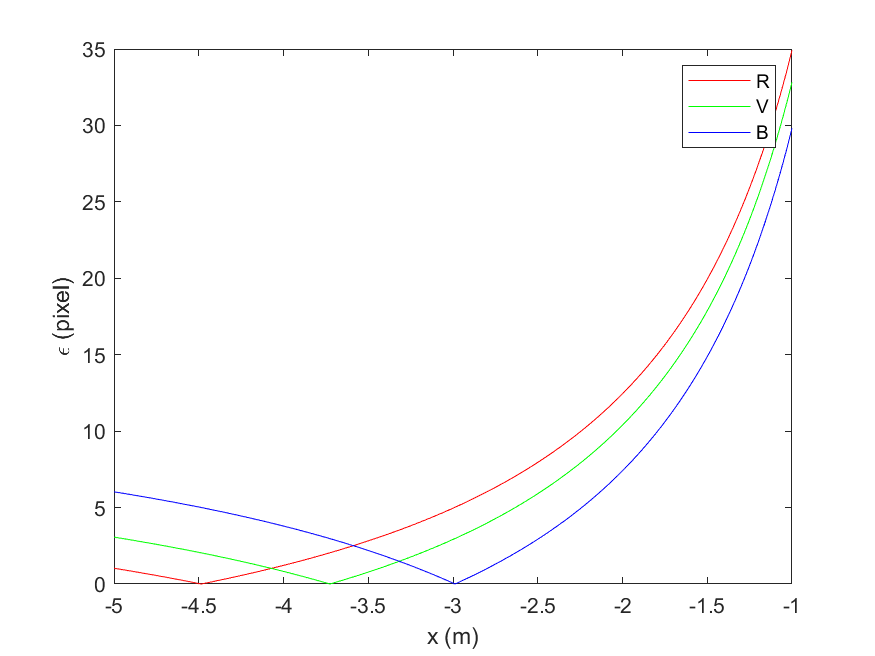
\includegraphics[width=0.4\textwidth]{Flou_optimise_capteur.png}
        \label{fig:edof-gdof}
    }
	\caption{Curvature radius optimization}
\end{figure}

%Further optimization can be achieved by adjusting the position of the detector. The optimal result for the pair \((R, x_0^{\prime})\) should be analyzed. This configuration will provide the best balance between chromatic aberration and image sharpness, enhancing the overall image quality.


\section{Conclusion}
We presented the post-processing algorithm and the corresponding optical design, and presented the optimization of that design. We saw the impact of the radius of curvature of a chromatic doublet onto the generalized depth of focus, taken as a criteria of image sharpness. The post-processing highlighted the High frequencies Transfer method, that equalized the depth of focus of the green and blue channels, resulting in a global R,G,B improved sharpness. Conceptually, post-processing algorithm will lead to better results when the GDOF is maximum, because a maximum of details (high frequencies components) will be resolved among the three color channels. So, if ones only want improve sharpness in the red spectrum, one can then maximize the red depth of foccus, regardless of the green's.

The optimization focused on two parameters, the radius of curvature between the two glasses, and the location of the detector. These two parameters enabled an enhancement of post-processed depth of focus of around 400\%.A possible way of improvement can be found in optical design courses, where correcting chromatic aberration often uses the right combination of glasses. Optimization can thus integrate material choices, and ultimately, conic parameters of surfaces too.

\pagebreak

\listoffigures

\end{document} 
